\documentclass[a4paper,12pt]{article}
\usepackage{geometry}
 \geometry{
 a4paper,
 total={170mm,257mm},
 left=20mm,
 top=20mm,
 }
\usepackage{verbatim}
\usepackage[utf8]{inputenc}
\usepackage{amsmath}
\usepackage{gensymb}
\usepackage{verbatim} % env for block comment 
\usepackage{ragged2e} % para usar flusleft
\usepackage[brazilian]{babel}
\usepackage{minted}
\usemintedstyle{tango}
\usepackage{graphicx}
\graphicspath{ {.} }

\begin{document}

\begin{center}
MAC5725 – Linguística Computacional\\
EP 1: Word2Vec\\
Wesley Seidel Carvalho\\
NUSP: 6544342\\
2020-02\\ %\hline
\end{center}

\begin{comment}
Este é um comentário de múltiplas linhas.
Com certeza útil para esconder partes grandes de texto ainda não revisadas.
Ou para encontrar um problema do seu código LaTeX que não compila.
\end{comment}

{\Large \textbf{EP1: Comentários} sobre a imagem gerada pelo programa}\\


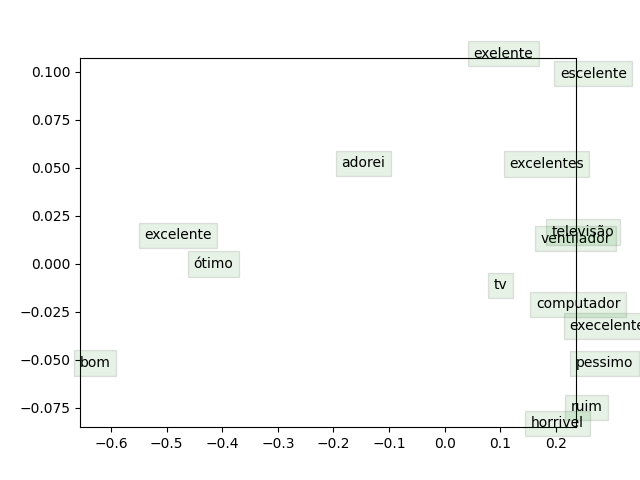
\includegraphics{vetores_de_palavras}

Em uma simples análise das posições das palavras na figura, podemos verificar que as palavras que expressam sentidos positivos e estão corretamente digitadas parecem obedecer uma reta ascendente que cruza o eixo vertical em -0,050. Além disso, outras palavras que apesar de estarem digitadas incorretamente, e que também expressam sentimento positivo(tais como exelente e escelente), estão acima do valor 0,025 no eixo vertical. Já as palavras que expressam sentimento negativos, estão bem difinidas abaixo do valor -0,030 no eixo vetical e acima de 0,15 do eixo horizontal. 

\end{document}